\subsubsection{Isabelle Overview}

Isabelle is a generic platform for tools based on formal logic.
It is generally known for its Isabelle/HOL library, which provides many theories and add-on tools (implemented in Isabelle/ML) in its \texttt{Main} theory and the \texttt{main} group of library sessions.
Some other (much smaller) Isabelle logics are FOL, LCF, ZF, CTT (an old version of Martin-L\"of Type Theory), but today most Isabelle applications are based on HOL.
The foundations of Isabelle due to Paulson~\cite{paulson700} are historically connected to \emph{logical frameworks} like Edinburgh LF: this fits nicely to the LF theory used in logic formalizations in MMT.
User contributions are centrally maintained in AFP, the \emph{Archive of Formal Proofs} (\url{https://www.isa-afp.org}).

From a high-level perspective, Isabelle is better understood as \emph{document-oriented proof assistant} or \emph{document preparation system} for domain-specific formal languages~\cite{Wenzel:IIdsflitd18}.
It allows flexible nesting of sub-languages, and types, terms, propositions, and proofs (in Isabelle/Isar) are merely a special case of that.
The result of processing Isabelle document sources consists of internal data structures in Isabelle/ML that are private to the language implementations.
Thus it is inherently difficult to observe Isabelle document content by external tools, e.g.\ to see which $\lambda$-terms occur in nested sub-languages.

Isabelle/PIDE \cite{Wenzel:2014:ITP-PIDE}, the Prover IDE framework, integrates all
activities of development for proofs and programs into a
\emph{semantic editor} Isabelle/jEdit. While the user is composing
text, the prover provides real-time feedback about its meaning: that
rich PIDE markup information can be rendered as conventional GUI
metaphors (e.g.\ text color, squiggly underline, tooltips, hyperlinks,
icons in the border) \cite{Wenzel:2019:MKM}. It is also possible to
run Isabelle/PIDE in ``headless mode'', to let some Isabelle/Scala
program observe markup as a formal library is processed in
Isabelle/ML.

The standard distribution of Isabelle\footnote{\url{https://isabelle.in.tum.de}} includes the
Isabelle/HOL library with various applications, but the main bulk of
applications is in the \emph{Archive of Formal Proofs}
(AFP)\footnote{\url{https://www.isa-afp.org}}, which is organized like
a scientific online journal. In August 2019, Isabelle/AFP had 492
articles by 331 authors, comprising 120\,MB source text total. Formal
checking requires approx.\ 50h CPU time or 2h elapsed time on high-end
multicore hardware. The result is a collection of heap images for the
internal state of Isabelle/ML and some HTML or PDF documents that
resemble conventional mathematical texts (with relatively little
formal markup being used here).


% % % % % % % % % % % % % % % % % % % % % % % % % % % % % % % % % % % % % % % % % % % % % % % % % % %
\subsubsection{General Technical Aspects of Exporting Isabelle Knowledge Bases}

Isabelle/ML is the \emph{internal implementation language} for logic-based tools, has direct access to the inference kernel in the manner of the ``LCF-approach'' \cite{Gordon-Milner-Wadsworth:1979}.
Isabelle/Scala is the \emph{external interface language} to manage Isabelle processes and
resulting content: it has access to the physical world with GUI frameworks, TCP servers, database engines etc.

To support exports like ours systematically, Wenzel had previously already instrumented the theory processing in Isabelle/ML to allow arbitrary \emph{presentation} for every theory node as it is finished: an ML function gets access to all commands with their intermediate theory
values; it can extract suitable information and \emph{export} it via a private channel to Isabelle/Scala.
The standard configuration of Isabelle provides options like \verb,export_theory, or \verb,export_proofs, to externalize certain aspects of theory content as a \emph{session database}.
For example, see command-line tools like \verb,isabelle build -o export_theory HOL-Analysis, to build such a database (for SQLite) and \verb,isabelle export -l HOL-Analysis, to query it later on.

Isabelle/Scala provides direct access to session builds and their results as an API for \emph{typed functional-object-oriented programming}: this is more robust and versatile than command-line tools.
For our export, we use the Isabelle/Scala APIs to provide dedicate command-line \verb,isabelle mmt_import,: options and arguments similar to \verb,isabelle build, specify a collection of sessions to be processed, the results are given to the MMT Scala API to write files in OMDoc format; there is extra output of RDF/XML files.

Our export (Isabelle repository version e6fa4b852bf9) turns this content into OMDoc and RDF/XML.
Our command-line tool uses regular Scala APIs of MMT (without intermediate files), and results are written to the file-system in OMDoc and RDF/XML format.
It runs a Prover IDE session (PIDE) under program control: a collection of \emph{sessions} with corresponding \emph{theories} is turned into formal source edits that are given to Isabelle/PIDE for semantic processing; the underlying prover process continuously produces markup reports as it explores the meaning of the source.
Whenever some theory node (with all imports) is finished, a separate Scala operation is invoked to \emph{commit} the result as
PIDE \emph{document snapshot}.
Thus the application can harvest theory exports produced up to that point, and the system can edit-out already processed theory-subgraphs to free resources, while the overall process is still running.

Thus the full material of AFP (hundreds of sessions, thousands of theories) can be digested on a high-end multicore machine within
approx. 24h elapsed time using 60 GB RAM for Isabelle/ML and 30 GB RAM for Isabelle/Scala.
This is approximately a factor 10 more than a conventional batch build, but the PIDE session is able to ``see'' more detailed information about the formal meaning of the sources (e.g.\ the use of term constants within the theory text, like the IDE front-end uses to provide hyperlink operations).

% % % % % % % % % % % % % % % % % % % % % % % % % % % % % % % % % % % % % % % % % % % % % % % % % % %
\subsubsection{Exporting Symbolic Knowledge in OMDoc/MMT Format}

We export all \emph{logical foundations} of theory documents (types, consts, facts, but \emph{not} proof terms), and aspects of \emph{structured specifications} (or ``little theories'') (locales and locale interpretations, which also subsumes the logical content of type classes).
Figure~\ref{fig:isabellemmt} shows a screenshot of the MMT browser showing a small part (the definition of binomial coefficients in Isabelle/HOL) of the exported Isabelle knowledge base.

\begin{figure}[ht]
  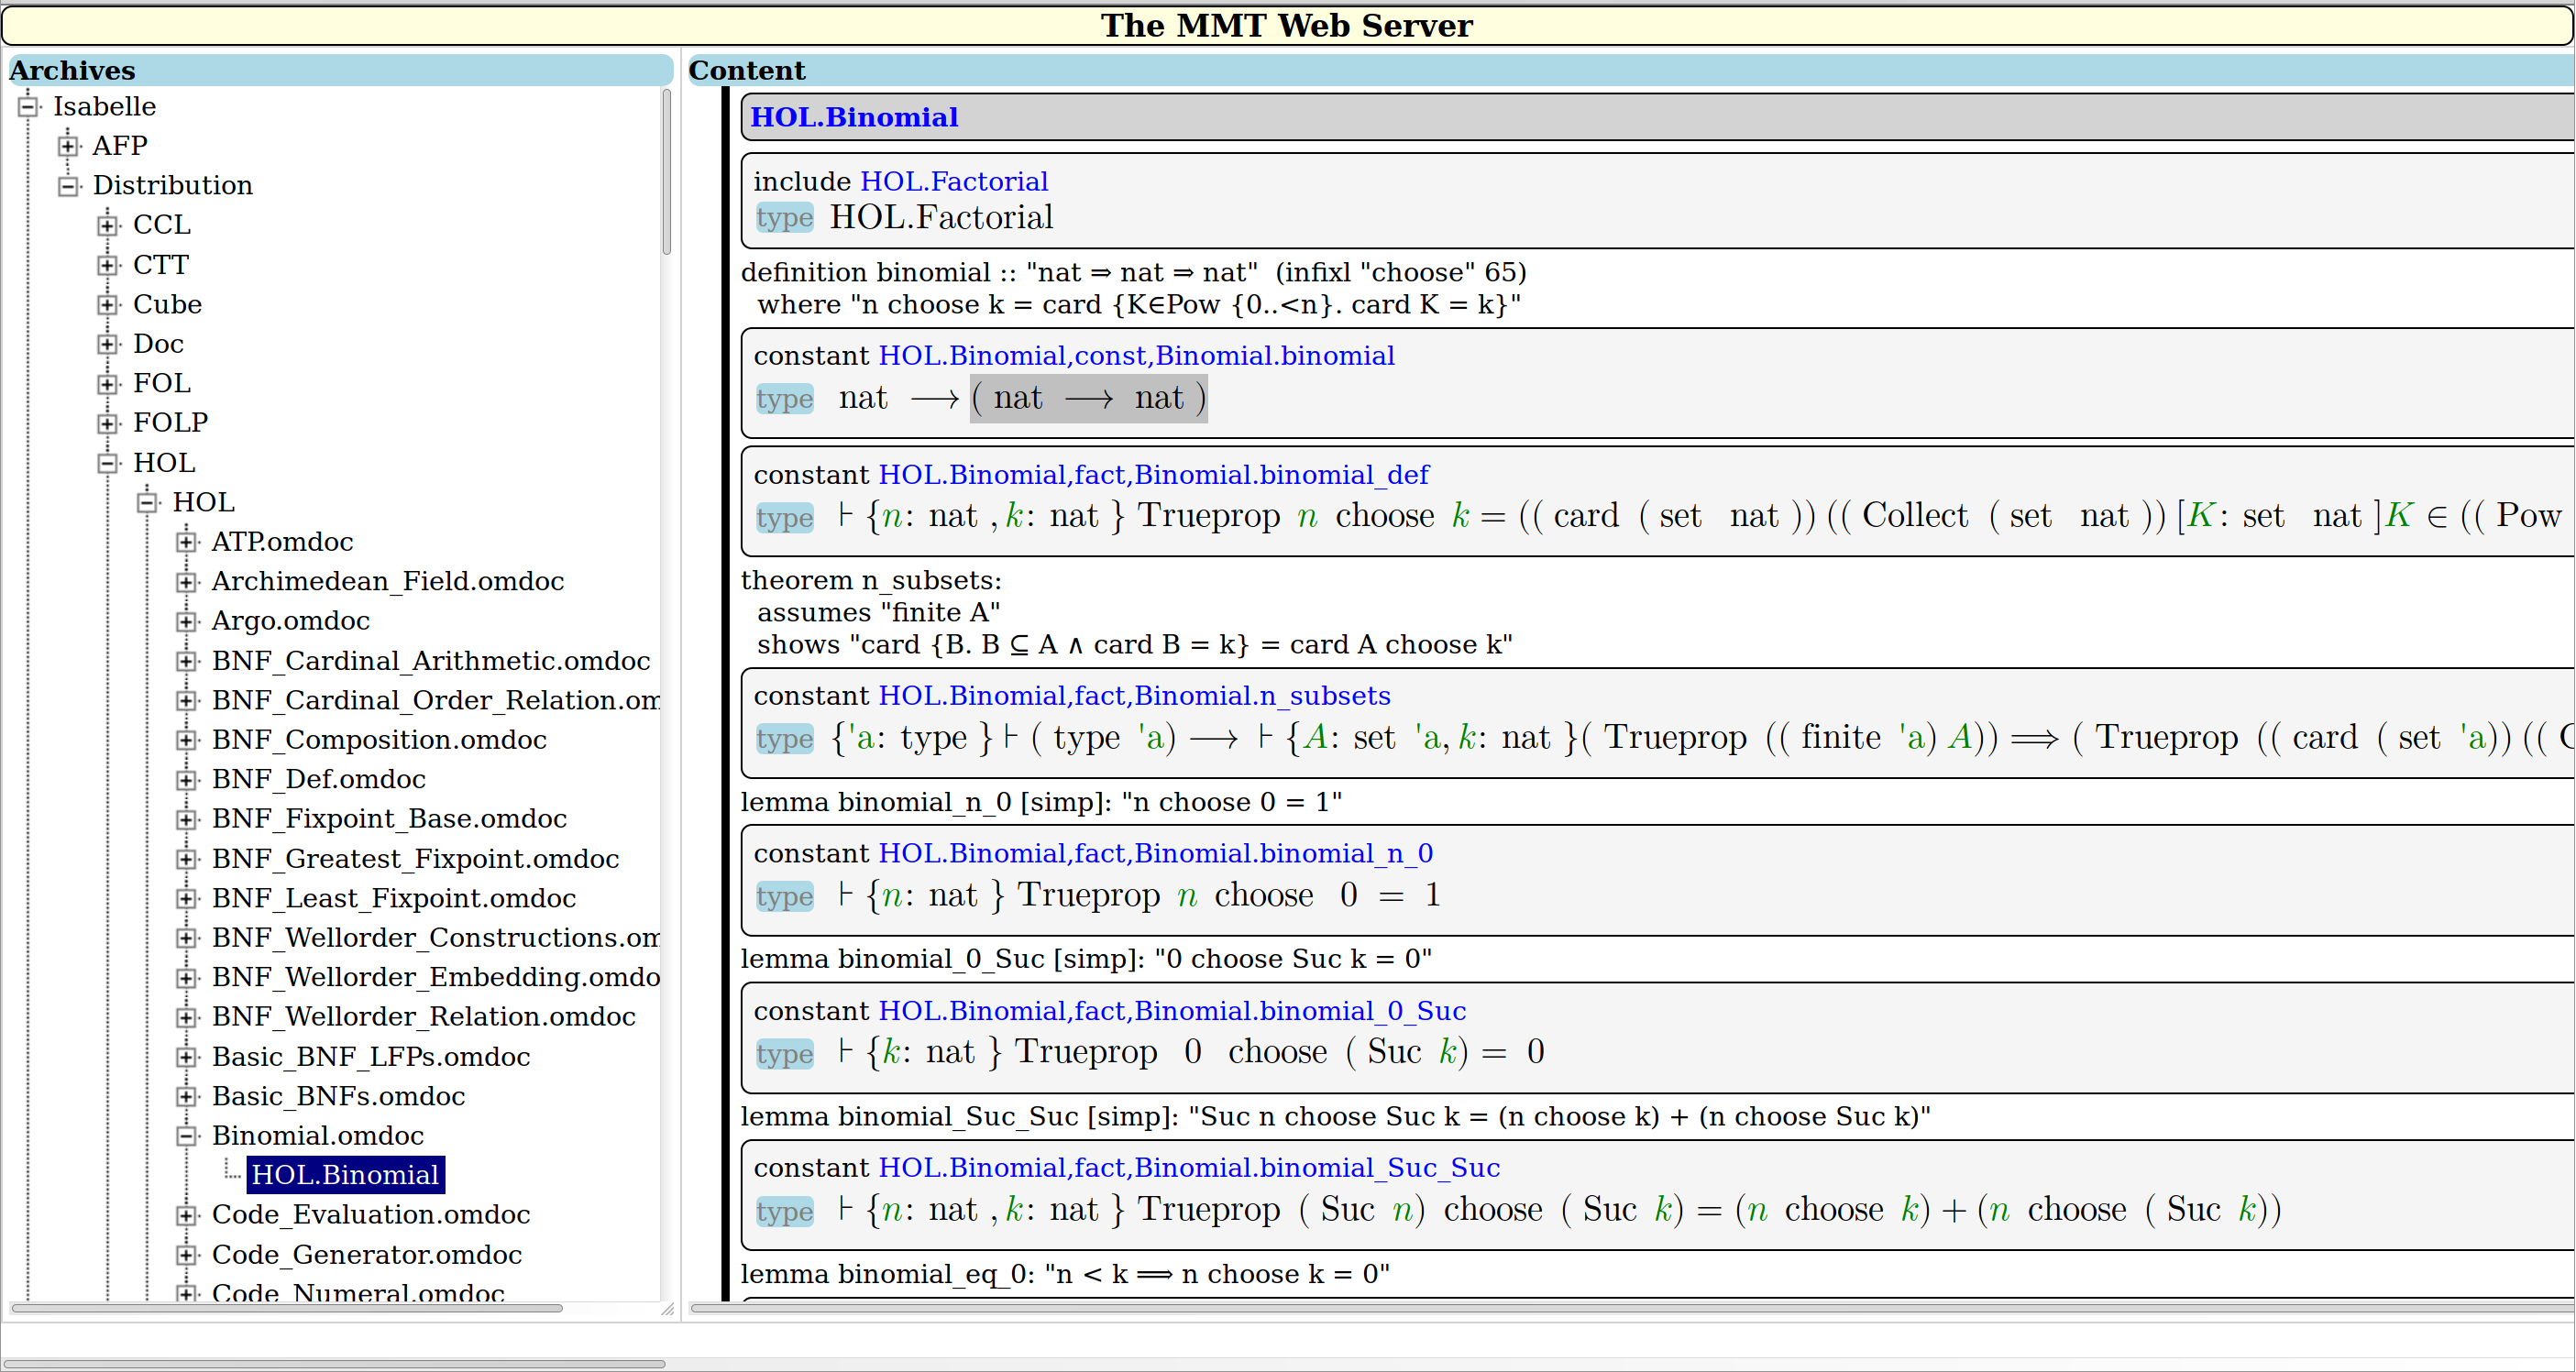
\includegraphics[width=\textwidth]{isabelle_mmt}
  \caption{MMT browser showing Isabelle content}\label{fig:isabellemmt}
\end{figure}

\paragraph{Module System}
All module system--level Isabelle entities are represented as MMT theories and morphisms.
These use a manually written MMT meta-theory that formalizes Isabelle/Pure --- the logic underlying Isabelle.

Besides plain Isabelle theories, this includes the order-sorted algebra of \emph{type classes} (subclass relation) and \emph{type arities} (image behavior of type constructors wrt.\ type class domains and ranges) in the sense of Nipkow and Prehofer \cite{Nipkow-Prehofer:1993} as well as locales in the sense of Ballarin \cite{Ballarin2014} and type classes as special locale interpretations in the sense of Haftmann and Wenzel \cite{Haftmann-Wenzel:2006:classes,Haftmann-Wenzel:2009}.

  Isabelle locales are \emph{named contexts} with type parameters
  (implicit), term parameters (\textbf{fixes}), and premises
  (\textbf{assumes}). Within such a ``little theory'' it is possible
  to spell out definitions, statements, proofs as usual --- all
  results are understood as relative to the context. The foundations
  will contain an extra prefix of type variables, term abstractions
  and assumptions according to the context.

  The export of locales preserves some of its internal structure,
  notably the locale dependency relation stemming from the
  construction of locales and sub-locales (by definition), as well as
  later locale interpretations (by proof).

  Type classes are special locales with a single type parameter and a
  canonical locale interpretation to connect \emph{type class
    parameters} (polymorphic constants with class constraints) to
  \emph{locale parameters} (fixed variables of the context). The
  export shows the result of the interpretation, but \emph{without} an
  explicit report on their connection.


\paragraph{Declarations}
Every declaration in a theory-like scope is represented as an MMT declaration.
This includes \textbf{types} (base types and type constructors),
  term \textbf{constants} (including functions, binders, quantifiers
  as higher-order constants), \textbf{axioms} (including equational
  axioms that count as primitive definitions), and \textbf{theorems}
  (propositions with a proof).

Isabelle definitions become equational axioms in MMT.
This includes theorems, which are treated as defined constants in MMT via the Curry-Howard representation.
However, the actual proofs, which become the definientia of these constants, are not exported by default (proof terms are prohibitively large), but it is possible to reconstruct the source text in the Isabelle/Isar proof language from the position information.

Type definitions in the sense of Gordon and
  Pitts \cite{pitts93} are interpreted
  definitionally within the standard semantics of the HOL
  logic. The export facility provides access to the key
  information: the old representing type, the new abstract type, the
  name of the morphisms between the two with the axiom stating the
  relation.
  This information allows recovering HOL typedefs faithfully, where
  Isabelle/Pure theory content would only show the individual
  particles. It also serves as an example to ``query'' derived
  specification mechanisms in Isabelle/ML, to expose its own level of
  abstraction to the exporter.
  
Term constants with indication of derived specifications
  mechanisms, e.g.\ \textbf{primrec} functions, \textbf{inductive} or
  \textbf{coinductive} relations are handled by querying generic
  information in Isabelle/Pure about functional or relation
  specifications (so-called ``Spec Rules''). The Isabelle/HOL
  implementations provide this data on their own account.

\paragraph{Expressions}
The expressions of Isabelle's $\lambda$-calculus are represented as MMT terms.
This part of the translation is relatively straightforward and similar to previous exports to OMDoc/MMT (e.g., \cite{KalRab:hollight:14,KohMueOwr:mpagsiuf17,MueRabSac:cltg19}).
Only the treatment of variables warrants further description, and we focus on it in the sequel.

Isabelle variables come in various flavours: free variables (e.g.\
\verb,x,), schematic variables with index (e.g. \verb,?x10,) and bound
variables (e.g. \verb,x, in $\lambda$\verb,x::,$\tau$\verb,. x, which
is concrete syntax for the de-Bruijn index abstraction
\verb;Abs (x, ;$\tau$\verb;, B.0); where \verb,x, is retained as a
comment). To fit smoothly into the lambda-calculus of MMT, variable
names are standardized as follows:

Schematic variables are renamed to fresh free variables. Since
  schematic variables are morally like a universal quantifier prefix,
  this preserves the logical meaning of a formala (e.g.\ a theorem
  statement).

Bound variable comments in abstractions are renamed locally to
  avoid clashes with free variables in the same scope. Thus the
  comment can be used literally in MMT/LF as named abstraction,
  ignoring the unnamed de-Bruijn index representation of Isabelle.

Finally, Isabelle type variables are decorated with type class constraints,
e.g.\ \verb,'a::order, for types that belong to the class \verb,order,
defined in the Isabelle/HOL library (e.g.\ \verb,nat, with its
standard order): this ensures certain \emph{operations} with a link to
overloaded term constants (e.g.\ \verb,less :: 'a => 'a => bool,), as
well as logical \emph{premises} on these operations (e.g.\ stating
that \verb,less, is a strict order on the type).

Isabelle class operations are managed by extra-logical means, e.g.\ by
the code-generator for Haskell or Standard ML, to produce the expected
\emph{dictionary construction} to eliminate the implicit
overloading. In MMT this will merely result in uncontrolled
polymorphism: constant definitions consist of multiple
(non-overlapping) equational specifications depending on the type
argument.

Isabelle class premises become logical constraints in a
straight-forward manner: a type class is a predicate over types in LF,
so \verb,'a::c, means that the predicate \verb,c, applied to type
\verb,'a, holds. Statements with class constraints
$\phi($\verb,'a::c,$)$ are augmented by a prefix of preconditions
\verb,'a::c,${} \Longrightarrow \phi($\verb,'a,$)$, effectively
eliminating the constraint within the logic.

\paragraph{Identifiers}
Isabelle constants live in separate name spaces (for types, terms,
theorems etc.).  For example, there could be a type \verb,Nat.nat, and
a term constant of the same name (e.g.\ an operation to make a natural
number). Qualification is usually by the theory \emph{base} name, not
the session-qualified long name; in rare situations, there is no
theory qualification at all. In order to have all entities coexist
within one big space of individuals in MMT, we use a triple that
consists of (\emph{long-theory-name}, \emph{entity-name},
\emph{entity-kind}) written as URI like as follows:

\begin{quote}
\texttt{https://isabelle.in.tum.de?}\emph{long-theory-name}\texttt{?}\emph{entity-name}\texttt{|}\emph{entity-kind}
\end{quote}

\noindent For example, \texttt{https://isabelle.in.tum.de?HOL.Nat?Nat.nat|type} refers to the type of natural numbers in the Isabelle/HOL library.


% % % % % % % % % % % % % % % % % % % % % % % % % % % % % % % % % % % % % % % % % % % % % % % % % % %
\subsubsection{Exporting Relational Knowledge in ULO Format}

Relations between formal items are output as RDF/XML triples,
  bypassing MMT and its OMDoc format; see also
  \cite[\S3.1]{ConKohMue:rdaml19}.  This also captures some aspects of
  inductive and primitive recursive definitions via
  \verb,ulo:inductive-on,. In addition to that paper, there is now
  full coverage of theorem dependencies via \verb,ulo:uses,, spanning
  a rather large dependency graph over the source text: it relates
  theorem statements with used constants and proofs with used
  theorems.  



\paragraph{Individuals}
Formal entities are identified by their \emph{name} and \emph{kind} as follows:
\begin{compactitem}
\item The name is a long identifier (with dot as separator, e.g.\ \texttt{Nat.Suc}) that is unique within the current theory context (including the union of all theory imports). Long names are managed by namespaces within the formal context to allow partially qualified names in user input and output (e.g.\ \texttt{Suc}). The structure of namespaces is known to the prover, and not exported.
\item The kind is a short identifier to distinguish the namespaces of formal entities, e.g.\ \texttt{type} for type constructors, \texttt{const} for term constants, \texttt{fact} for lists of theorems that are recorded in the context, but also non-logical items like \texttt{method} (Isar proof methods), \texttt{attribute} (Isar hint language) etc.
\end{compactitem}

\noindent
This name/kind scheme is in contrast to usual practice in universal $\lambda$-calculus representations like MMT/LF, e.g.\ there could be a type \texttt{Nat.nat} and a separate term constant of the same name.  Moreover the qualification in long names only uses theory base names, not their session-qualified long name (which was newly introduced in Isabelle2017). So in order to support one big space of individuals over all Isabelle sessions and theories, we use the URI format that was already used for identifiers above.

\paragraph{Logic}
The primitive logical entities of Isabelle/Pure are types, terms, and theorems (facts).
Additionally, Isabelle supports various theory-like structures.
These correspond our declaration classes as follows:
\begin{compactitem}
\item \ind{theory} refers to global \textbf{theory} and local \textbf{locale} contexts. There are various derivatives of \textbf{locale} that are not specifically classified, notably \textbf{class} (type classes) and \textbf{experiment} (locales with inaccessible namespace).
\item \ind{type} refers to \emph{type constructors} of Isabelle/Pure, and object-logic types of many-sorted FOL or simply-typed HOL. These types are syntactic, and not to be confused with the ``propositions-as-types'' approach in systems like Coq. Dependent types are represented as terms in Isabelle.
\item \ind{function} refers to \emph{term constants}, which are ubiquitous in object-logics and applications. This covers a broad range of formal concepts, e.g.\ logical connectives, quantifiers (as operators on suitable $\lambda$-terms), genuine constants or mathematical functions, but also recursion schemes, or summation, limit, integration operators as higher-order functions.
\item \ind{statement} refers to individual theorems, which are projections from the simultaneous \texttt{fact} lists of Isabelle.  Only the head statement of a theorem is considered, its proof body remains abstract (as reference Isar to proof text).
Theorems that emerge axiomatically (command \textbf{axiomatization}) are marked as \ind{primitive}, properly proven theorems as \ind{derived}, and theorems with unfinished proofs (command \textbf{sorry}) as \ind{experimental}.
\end{compactitem}

\noindent The \ind{specifies} and \ind{specified-in} relations connect theories and locales with their declared individuals.
The \ind{uses} relation between those represents syntactic occurrence of individuals in the type (or defining term) of formal entities in Isabelle: it spans a large acyclic graph of dependencies. Again, this excludes proofs: in principle there could be a record of individuals used in the proof text or by the inference engine, but this is presently unimplemented.

The \ind{source-ref} property refers to the defining position of formal entities in the source.
Thanks to Isabelle/PIDE, this information is always available and accurate: the Prover IDE uses it for highlighting and hyperlinks in the editor view. Here we use existing URI notation of MMT, e.g.\ \url{https://isabelle.in.tum.de/source/FOL/FOL/FOL.theory#375.19.2:383.19.10} with offset~/ line~/ column of the two end-points of a text interval.

The \ind{check-time} and \ind{external-size} properties provide some measures of big theories in time (elapsed) and space (sources).  This is also available for individual commands, but it is hard to relate to resulting formal entities: a single command may produce multiple types, consts, and facts simultaneously.

\paragraph{Semi-formal Documents}
We use \ind{section} for the six levels of headings in Isabelle documents: \textbf{chapter}, \textbf{section}, \dots, \textbf{subparagraph}.  These are turned into dummy individuals (which are counted consecutively for each theory).

\ind{file}, \ind{folder}, \ind{library} are presently unused.
They could refer to the overall project structure Isabelle document sources in the sense of~\cite{Wenzel:IIdsflitd18}, namely as \emph{theories} (text files), \emph{sessions} (managed collections of theories), and \emph{project directories} (repository with multiple session roots).

For document metadata, we use the Dublin Core ontology.  The Isabelle command language has been changed to support a new variant of \emph{formal comment}. With one keystroke, the presentation context of a command may be augmented by arbitrary user-defined marker expressions. Isabelle/Pure already provides \texttt{title}, \texttt{creator}, \texttt{contributor} etc.\ from \S\ref{sec:objprops}: they produce PIDE document markup that Isabelle/MMT can access and output as corresponding RDF.

This approach allows to annotate theory content \emph{manually}: a few theories of \texttt{HOL-Algebra} already use the new feature sporadically. For automatic marking, metadata of AFP entries is re-used for their theories. One could also digest comments in theory files about authors, but this is presently unimplemented.


\subsubsection{Statistics}\label{sec:stats}

We present some statistics\footnote{Versions: Isabelle/9c60fcfdf495, AFP/d50417d0ae64, MMT/e6fa4b852bf9.}.
This gives an idea about overall size and scalability of the export facilities so far.
The datasets are publicly available from \url{https://gl.mathhub.info/Isabelle}.

{\tiny
\begin{center}
\begin{tabular}{cl||r|r||r|r|r|r|r||r|r}
  & Library                       & Individuals & Relations  & Theories & Locales  & Types      & Constants & Statements  & RDF/XML    & elapsed \\
  &                               &             &            &          &          &            &           &             & file size  & time \\\hline
  \isabelle & Distribution        &     103,873 &  2,310,704 &      535 &     496  &   235      & 8,973     &     88,960  & 188\,MB    & 0.5h \\
            & only group                                                                                                    
                    \texttt{main} &             &            &          &          &            &           &             &            & \\\hline
  \isabelle & Distribution+AFP    &   1,619,889 & 36,976,562 &    6,185 &  4,599   & 10,592     & 215,878   &  1,359,297  & 3,154\,MB  & 16.5h \\
            & without \verb,very_slow,
                                  &             &            &          &          &            &           &             &            & \\\hline
%  \coq      & All 49 Libraries    & 383,527     & 11,516,180 &    1,979 & -        &  6,061     & -         &  161,736    & 452\,MB    & \\
\end{tabular}
\end{center}}

%%% Local Variables:
%%% mode: latex
%%% mode: visual-line
%%% fill-column: 5000
%%% TeX-master: "report"
%%% End:

%  LocalWords:  subsubsection texttt texttt paulson700 emph Wenzel:IIdsflitd18 organized verb,export_theory verb,export_proofs externalize verb,isabelle verb,isabelle consts fig:isabellemmt includegraphics textwidth isabelle_mmt arities wrt Prehofer Nipkow-Prehofer:1993 Ballarin Ballarin2014 textbf pitts93 primrec coinductive ednote pvs verb,x verb,order verb,nat verb,less verb,c Longrightarrow noindent ConKohMue:rdaml19 verb,ulo:inductive-on verb,ulo:uses compactitem axiomatization sec:objprops hline verb,very_slow formalizations KohMueOwr:mpagsiuf17,MueRabSac:cltg19 standardized
